\documentclass{book}


%%% packages %%%
\usepackage{color}
\usepackage{ulem}
\usepackage{amsmath}
\usepackage{amssymb}
\usepackage{xfrac}
\usepackage{import}
\usepackage{listings}
\usepackage{hyperref}
\usepackage[inner=3cm, outer=3cm]{geometry}

%%% newcommands %%%
\newcommand{\abbas}{\textcolor[rgb]{0.65,0.92,0.14}{\textbf{\emph{ABBAS}}}}
\newcommand{\myc}{\noindent\textbf{{\color{blue} Code}:}}
\newcommand{\myo}{\noindent\textbf{{\color{blue} Output}:\\}}
\newcommand{\cool}[2]{{\colorbox{black}{{\color{red} #1}, {\color{green} #2}}}}


%%% renewcommands %%%
\renewcommand{\thefootnote}{\roman{footnote}}

%%% newenvironments %%%
\newenvironment{bb}
{
\begin{center}
\begin{tabular}{|p{0.9\textwidth}|}
\hline\\
}
{
\\\\\hline
\end{tabular}
\end{center}
}

%%% newtheorems %%%



%%% define color %%%
\definecolor{codegreen}{rgb}{0,0.6,0}
\definecolor{codegray}{rgb}{0.5,0.5,0.5}
\definecolor{codepurple}{rgb}{0.58,0,0.82}
\definecolor{backcolour}{rgb}{0.95,0.95,0.92}

%%% define style %%%
\lstdefinestyle{mystyle}{
    backgroundcolor=\color{backcolour},
    commentstyle=\color{codegreen},
    keywordstyle=\color{magenta},
    numberstyle=\tiny\color{codegray},
    stringstyle=\color{codepurple},
    basicstyle=\ttfamily\footnotesize,
    breakatwhitespace=false,
    breaklines=true,
    captionpos=b,
    keepspaces=true,
    numbers=left,
    numbersep=5pt,
    showspaces=false,
    showstringspaces=false,
    showtabs=false,
    tabsize=2
}

%%% set style %%%
\lstset{style=mystyle}


%%% document %%%
\begin{document}

\title{Getting Started with \LaTeX{}}
\author{
Abbas Yazdanmehr \\
Computer Engineering Faculty, Shahid Beheshti University \\
\texttt{abbas.yazdanmehr1@gmail.com}
}
\date{\today}

\maketitle

\tableofcontents


\chapter{Commands}\

\section{Article/Book Partitions}
\begin{enumerate}
  \item part
  \item chapter
  \item section
  \item subsection
  \item subsubsection
  \item paragraph
  \item subparagraph
\end{enumerate}

\section{Next Line}
see this line. \\
this is next line in \LaTeX.\\[1cm]
now see this line and compare the space to previous line. \\[2cm]
this is in continue of previous line.

\section*{Note}
for changing all of document space between lines you can use from linespread global command. for more complete spacing between lines and words you can use spacing package.\\

\section*{hfill}
\myc
\begin{lstlisting}
start of line \hfill end of line \\
start of line \hfill middle of line \hfill end of line\\
start \hfill $\frac{1}{4}$ \hfill middle \hfill $\frac{3}{4}$ \hfill end
\end{lstlisting}

\myo
start of line \hfill end of line \\
start of line \hfill middle of line \hfill end of line\\
start \hfill $\frac{1}{4}$ \hfill middle \hfill $\frac{3}{4}$ \hfill end

\section{noindent}
\noindent
Every where that you don't want first line indentation you can use noindent command.

\section{addvspace}
Consider this as first text,

\addvspace{2cm}
\noindent
This text is 2 centimeter lower than first text.
\smallskip
\noindent
This text has smallskip from previous.
\medskip
\noindent
This text has medskip from previous.
\bigskip
\noindent
This text has bigskip from previous.

\section{Size in Latex}
\myc
\begin{lstlisting}
{\tiny this is tiny} \\
{\scriptsize this is scriptsize} \\
{\footnotesize this is large} \\
{\small this is small} \\
{\normalsize this is normalsize}\\
{\large this is large}\\
{\Large this is Large}\\
{\LARGE this is LARGE}\\
{\huge this is huge}\\
{\Huge this is Huge}
\end{lstlisting}

\myo
{\tiny this is tiny} \\
{\scriptsize this is scriptsize} \\
{\footnotesize this is large} \\
{\small this is small} \\
{\normalsize this is normalsize}\\
{\large this is large}\\
{\Large this is Large}\\
{\LARGE this is LARGE}\\
{\huge this is huge}\\
{\Huge this is Huge}

\section{Text Styling}
\myc
\begin{lstlisting}
\noindent
\emph{this is emph} \\
\textbf{this is textbf} \\
\textrm{this is textrm} \\
\textsf{this is textsf} \\
\texttt{this is textt} \\
\textmd{this is textmd} \\
\textit{this is textit} \\
\textsc{this is textsc} \\
\textsl{this is textsl} \\
{\verb "this can't be a latex command"}
\end{lstlisting}

\myo
\noindent
\emph{this is emph} \\
\textbf{this is textbf} \\
\textrm{this is textrm} \\
\textsf{this is textsf} \\
\texttt{this is textt} \\
\textmd{this is textmd} \\
\textit{this is textit} \\
\textsc{this is textsc} \\
\textsl{this is textsl} \\
{\verb "this can't be a latex command"}

\section{Line On Text}
\myc
\begin{lstlisting}
\uline{this is uline} \\
\uuline{this is uuline} \\
\uwave{this is uwave} \\
\sout{this is sout} \\
\xout{this is xout} \\
\end{lstlisting}

\myo
\uline{this is uline} \\
\uuline{this is uuline} \\
\uwave{this is uwave} \\
\sout{this is sout} \\
\xout{this is xout} \\

\section{Text Color}
\myc
\begin{lstlisting}
\textcolor[rgb]{0.94,0.22,0.22}{this sentence is red.}\\
\textcolor{red}{also this is red again.}\\
\textcolor[rgb]{0.11,0.27,0.83}{this is blue.} \\
{\color{blue} this is blue and uses better command in code}\\
\end{lstlisting}

\myo
\textcolor[rgb]{0.94,0.22,0.22}{this sentence is red.}\\
\textcolor{red}{also this is red again.}\\
\textcolor[rgb]{0.11,0.27,0.83}{this is blue.} \\
{\color{blue} this is blue and uses better command in code}\\

\section{Text Background Color}
\myc
\begin{lstlisting}
\colorbox{yellow}{this text background color is yellow :).}
\end{lstlisting}

\myo
\colorbox{yellow}{this text background color is yellow :).}

\newpage
\section{Page Color}
\myc
\begin{lstlisting}
\pagecolor{green}
    {\color{red}
        this page is black my friend.\\
        if you use color globally all of page color change.\\
    }

\newpage
\nopagecolor
\end{lstlisting}

\myo
\pagecolor{green}
    {\color{red}
        this page is black my friend.\\
        if you use color globally all of page color change.\\
    }

\newpage
\nopagecolor


\newpage
\section{footnote}
\noindent
we are going to put a footnote mark right here \footnote{The footnote text goes here.} as a \LaTeX lesson.\\
\noindent
we are going to put a footnote mark right here \footnote{The footnote text goes here.} as a \LaTeX lesson.\\
\noindent
we are going to put a footnote mark right here \footnote{The footnote text goes here.} as a \LaTeX lesson.\\
\noindent
we are going to put a footnote mark right here \footnote{The footnote text goes here.} as a \LaTeX lesson.\\
\noindent
we are going to put a footnote mark right here \footnote{The footnote text goes here.} as a \LaTeX lesson.\\

\setcounter{footnote}{0}

\noindent
we are going to put a footnote mark right here \footnote{The footnote text goes here.} as a \LaTeX lesson.\\
\noindent
we are going to put a footnote mark right here \footnote{The footnote text goes here.} as a \LaTeX lesson.\\
\noindent
we are going to put a footnote mark right here \footnote{The footnote text goes here.} as a \LaTeX lesson.\\


\chapter{Environments}

\section{description}

\myc
\begin{lstlisting}
\begin{description}
  \item[item1] this is Item1 description
  \item[item2] this is item2 description
  \item[item3] this seems very cool no?
\end{description}
\end{lstlisting}

\noindent
\myo
\begin{description}
  \item[item1] this is Item1 description
  \item[item2] this is item2 description
  \item[item3] this seems very cool no?
\end{description}



\section{center}

\myc
\begin{lstlisting}
\begin{center}
  this text is the center of line\\
  also this is the center of line\\
  this is new line\\
  what you want?\\
  new line?
\end{center}
\end{lstlisting}

\myo
\begin{center}
  this text is the center of line\\
  also this is the center of line\\
  this is new line\\
  what you want?\\
  new line?
\end{center}

\section{itemize}
\myc
\begin{lstlisting}
\begin{itemize}
  \item this is first
  \item second
  \item third
  \item last
\end{itemize}
\end{lstlisting}

\myo
\begin{itemize}
  \item this is first
  \item second
  \item third
  \item last
\end{itemize}

\section{enumerate}
\myc
\begin{lstlisting}
\begin{enumerate}
  \item you can see number
  \item in the continue
  \item this is enumerate
\end{enumerate}
\end{lstlisting}

\myo
\begin{enumerate}
  \item you can see number
  \item in the continue
  \item this is enumerate
\end{enumerate}

\section{flushleft}
\myc
\begin{lstlisting}
\begin{flushleft}
  this is flush left you see this text from left to right
\end{flushleft}
\end{lstlisting}

\myo
\begin{flushleft}
  this is flush left you see this text from left to right
\end{flushleft}

\section{flushright}
\myc
\begin{lstlisting}
\begin{flushright}
  this is flush right you see this text from right to left
\end{flushright}
\end{lstlisting}

\myo
\begin{flushright}
  this is flush right you see this text from right to left
\end{flushright}

\section{verse}
\myc
\begin{lstlisting}
\begin{verse}
  this is verse,\\
  I write hiphop here,\\
  yeah, yeah, yeah,
\end{verse}
\end{lstlisting}

\myo
\begin{verse}
  this is verse,\\
  I write hiphop here,\\
  yeah, yeah, yeah,
\end{verse}

\section{minipage}
\myc
\begin{lstlisting}
\begin{minipage}{5cm}
  I write in minipage environment content (body part). I have no idea what is like this.
\end{minipage}
\end{lstlisting}

\myo
\begin{minipage}{5cm}
  I write in minipage environment content (body part). I have no idea what is like this.
\end{minipage}

\section{quote}
\myc
\begin{lstlisting}
\begin{quote}
  this is some quote from unknown man,\\ be human!
\end{quote}
\end{lstlisting}

\myo
\begin{quote}
  this is some quote from unknown man,\\ be human!
\end{quote}

\section{quotation}
\myc
\begin{lstlisting}
\begin{quotation}
  this is quotation environment\\ what is difference between this and previous?
\end{quotation}
\end{lstlisting}

\myo
\begin{quotation}
  this is quotation environment\\ what is difference between this and previous?
\end{quotation}

\section{verbatim}
\myc
\begin{lstlisting}
\begin{verbatim}
this is verbatim environment you see this part monospace and all word width are equal. \\
you can see the verbatim environment have automatic word wrap!\\
so if you want that you should use listings package.\\
in the verbatim environment you can't use latex command and environment,\\
see this: \phi
\end{verbatim}
\end{lstlisting}

\myo
\begin{verbatim}
this is verbatim environment you see this part monospace and all word width are equal. \\
you can see the verbatim environment have automatic word wrap!\\
so if you want that you should use listings package.\\
in the verbatim environment you can't use latex command and environment,\\
see this: \phi
\end{verbatim}

\section{array}
\myc
\begin{lstlisting}
$
\begin{array}{ccc}
  first & second & third \\
  something & chert & continue
\end{array}$
\end{lstlisting}
\myo
$
\begin{array}{ccc}
  first & second & third \\
  something & chert & continue
\end{array}
$





\section{tabular}
\myc
\begin{lstlisting}
\begin{tabular}{c|c}
\hline
0 & nonhereditariness \\
\hline
1 & nonheretical \\
\hline
2 & nonheretically \\
\hline
3 & nonheritability \\
\hline
4 & nonheritable \\
\hline
5 & nonheritably \\
\hline
6 & nonheritor \\
\hline
7 & nonhero \\
\hline
8 & nonheroes \\
\hline
\end{tabular}
\end{lstlisting}

\myo
\begin{tabular}{c|c}
\hline
0 & nonhereditariness \\
\hline
1 & nonheretical \\
\hline
2 & nonheretically \\
\hline
3 & nonheritability \\
\hline
4 & nonheritable \\
\hline
5 & nonheritably \\
\hline
6 & nonheritor \\
\hline
7 & nonhero \\
\hline
8 & nonheroes \\
\hline
\end{tabular}


\myc
\begin{lstlisting}
\begin{tabular}{|c|||c||c|}
    \hline
  1 & 2 & 3 \\
  \hline
  \hline
  \hline
  6 & 5 & 4 \\
  \hline
  \hline
  7 & 8 & 9 \\
  \hline
\end{tabular}
\end{lstlisting}

\myo
\begin{tabular}{|c|||c||c|}
    \hline
  1 & 2 & 3 \\
  \hline
  \hline
  \hline
  6 & 5 & 4 \\
  \hline
  \hline
  7 & 8 & 9 \\
  \hline
\end{tabular}


\myc
\begin{lstlisting}
\begin{tabular}{|l|l||l|}
  \hline
  some text & another text & third text \\
  \cline{1-1}
  \cline{3-3}
  4 & 5 & 6 \\
  \cline{1-2}
  7 & 8 & 9 \\
  \hline
\end{tabular}
\end{lstlisting}

\myo
\begin{tabular}{|l|l||l|}
  \hline
  some text & another text & third text \\
  \cline{1-1}
  \cline{3-3}
  4 & 5 & 6 \\
  \cline{1-2}
  7 & 8 & 9 \\
  \hline
\end{tabular}

\myc
\begin{lstlisting}
\begin{tabular}{|l|l|l|}
  \hline
  \multicolumn{2}{|l|}{some text} & 0 \\
  \hline
  1 & 2 & 3 \\
  \hline
  1 & 2 & 3 \\
  \hline
\end{tabular}
\end{lstlisting}

\myo
\begin{tabular}{|l|l|l|}
  \hline
  \multicolumn{2}{|l|}{some text} & 0 \\
  \hline
  1 & 2 & 3 \\
  \hline
  1 & 2 & 3 \\
  \hline
\end{tabular}

\myc
\begin{lstlisting}
\begin{tabular}{|c|c|c|c|p{5cm}|}
  \hline
  1 & 2 & 3 & 4 & This Macro Manual describes all WinEdt macro functions. Elements, rules and syntax of the macro language are described in depth. \\
  \hline
  1 & 2 & 3 & 4 & Most WinEdt menu items consist of a sequence of predefined macro functions separated by a semicolon ";". \\
  \hline
  1 & 2 & 3 & 4 & However, more sophisticated macros (e.g. Insert n x m Array) are normally defined in macro scripts. \\
  \hline
\end{tabular}
\end{lstlisting}
\myo
\begin{tabular}{|c|c|c|c|p{5cm}|}
  \hline
  1 & 2 & 3 & 4 & This Macro Manual describes all WinEdt macro functions. Elements, rules and syntax of the macro language are described in depth. \\
  \hline
  1 & 2 & 3 & 4 & Most WinEdt menu items consist of a sequence of predefined macro functions separated by a semicolon ";". \\
  \hline
  1 & 2 & 3 & 4 & However, more sophisticated macros (e.g. Insert n x m Array) are normally defined in macro scripts. \\
  \hline
\end{tabular}


\section{equation}
\section*{(mathematic mode explain here!)}
\myc
\begin{lstlisting}
\begin{equation}\label{eq.secondlaw}
  F = m a\:.
\end{equation}
\end{lstlisting}


\myo
\begin{equation}\label{eq.secondlaw}
  F = m a\:.
\end{equation}

\myc
\begin{lstlisting}
\begin{equation}\label{eq.greeks}
  \alpha \beta \lambda \mu \epsilon
\end{equation}
\end{lstlisting}

\myo
\begin{equation}\label{eq.greeks}
  \alpha \beta \lambda \mu \epsilon
\end{equation}

\myc
\begin{lstlisting}
\begin{equation}
  \frac{a}{b} \times \frac{c}{d}=\frac{a \times c}{b \times d}
\end{equation}
\end{lstlisting}

\myo
\begin{equation}
  \frac{a}{b} \times \frac{c}{d}=\frac{a \times c}{b \times d}
\end{equation}


\myc
\begin{lstlisting}
\begin{equation}\label{eq.frac2}
  \frac{a}{1 + \frac{b}{c}}
\end{equation}
\end{lstlisting}

\myo
\begin{equation}\label{eq.frac2}
  \frac{a}{1 + \frac{b}{c}}
\end{equation}


\myc
\begin{lstlisting}
\begin{equation}\label{eq.sfrac}
  \sfrac{a}{b}
\end{equation}
\end{lstlisting}

\myo
\begin{equation}\label{eq.sfrac}
  \sfrac{a}{b}
\end{equation}


\myc
\begin{lstlisting}
\begin{equation}\label{eq.golden}
  \phi = \frac{1+\sqrt{5}}{2}
\end{equation}
\end{lstlisting}

\myo
\begin{equation}\label{eq.golden}
  \phi = \frac{1+\sqrt{5}}{2}
\end{equation}


\myc
\begin{lstlisting}
\begin{equation}\label{eq.combination}
  \binom{n}{m} = \frac{n!}{m!(n-m)!}
\end{equation}
\end{lstlisting}

\myo
\begin{equation}\label{eq.combination}
  \binom{n}{m} = \frac{n!}{m!(n-m)!}
\end{equation}

\section{displaymath}
\myc
\begin{lstlisting}
\begin{displaymath}
  this is math mode in \int_{2}^{3} f(x) + g(x) dx
\end{displaymath}
\end{lstlisting}

\myo
\begin{displaymath}
  this is math mode in \int_{2}^{3} f(x) + g(x) dx
\end{displaymath}

\section{inline math}
\myc
\begin{lstlisting}
this is $x^2\sqrt{x}$ and this is $\mathbf{x}$ for mathematics inline.
\end{lstlisting}

\myo
this is $x^2\sqrt{x}$ and this is $\mathbf{x}$ for mathematics inline.

\myc
\begin{lstlisting}
\begin{equation}\label{eq.paranthes}
    \left( \right)
\end{equation}
\end{lstlisting}

\myo
\begin{equation}\label{eq.paranthes}
    \left( \right)
\end{equation}


\myc
\begin{lstlisting}
\begin{equation}\label{eq.matrix1}
  \mathbf{A} = \left(\begin{array}{cc|c}
                        1 & 2 & 3 \\
                        4 & 5 & 6 \\
                        \hline
                        7 & 8 & 9
                     \end{array}
                     \right)
\end{equation}
\end{lstlisting}

\myo
\begin{equation}\label{eq.matrix1}
  \mathbf{A} = \left(\begin{array}{cc|c}
                        1 & 2 & 3 \\
                        4 & 5 & 6 \\
                        \hline
                        7 & 8 & 9
                     \end{array}
                     \right)
\end{equation}

\myc
\begin{lstlisting}
\begin{equation}\label{eq.matrix0}
  \mathbf{A} = \begin{bmatrix}
                        1 & 2 & 3 \\
                        4 & 5 & 6 \\
                        7 & 8 & 9
                     \end{bmatrix}
\end{equation}
\end{lstlisting}

\myo
\begin{equation}\label{eq.matrix0}
  \mathbf{A} = \begin{bmatrix}
                        1 & 2 & 3 \\
                        4 & 5 & 6 \\
                        7 & 8 & 9
                     \end{bmatrix}
\end{equation}

\myc
\begin{lstlisting}
\begin{equation}\label{eq.matrix2}
  \mathbf{A} = \begin{pmatrix}
                        1 & 2 & 3 \\
                        4 & 5 & 6 \\
                        7 & 8 & 9
                     \end{pmatrix}
\end{equation}
\end{lstlisting}

\myo
\begin{equation}\label{eq.matrix2}
  \mathbf{A} = \begin{pmatrix}
                        1 & 2 & 3 \\
                        4 & 5 & 6 \\
                        7 & 8 & 9
                     \end{pmatrix}
\end{equation}

\myc
\begin{lstlisting}
\begin{equation}\label{eq.matrix2}
  \mathbf{A} = \begin{vmatrix}
                        1 & 2 & 3 \\
                        4 & 5 & 6 \\
                        7 & 8 & 9
                     \end{vmatrix}
\end{equation}
\end{lstlisting}

\myo
\begin{equation}\label{eq.matrix2}
  \mathbf{A} = \begin{vmatrix}
                        1 & 2 & 3 \\
                        4 & 5 & 6 \\
                        7 & 8 & 9
                     \end{vmatrix}
\end{equation}

\myc
\begin{lstlisting}
\begin{equation}\label{eq.matrix3}
  \mathbf{A} = \begin{Vmatrix}
                        1 & 2 & 3 \\
                        4 & 5 & 6 \\
                        7 & 8 & 9
                     \end{Vmatrix}
\end{equation}
\end{lstlisting}

\myo
\begin{equation}\label{eq.matrix3}
  \mathbf{A} = \begin{Vmatrix}
                        1 & 2 & 3 \\
                        4 & 5 & 6 \\
                        7 & 8 & 9
                     \end{Vmatrix}
\end{equation}

\myc
\begin{lstlisting}
\begin{equation}\label{eq.matrix4}
  \bordermatrix{~ & a & b \cr
                c & 1 & 2 \cr
                d & 3 & 4 \cr}
\end{equation}
\end{lstlisting}

\myo
\begin{equation}\label{eq.matrix4}
  \bordermatrix{~ & a & b \cr
                c & 1 & 2 \cr
                d & 3 & 4 \cr}
\end{equation}


\section{align}
\myc
\begin{lstlisting}
\begin{align}\label{al.01}
  E &= K + U \\
  K &= \sfrac{1}{2} \;m v^2 \\
  U &= mgh
\end{align}
\end{lstlisting}

\myo
\begin{align}\label{al.01}
  E &= K + U \\
  K &= \sfrac{1}{2} \;m v^2 \\
  U &= mgh
\end{align}

\section{figure}
\myc
\begin{lstlisting}
\begin{figure}
  \centering
  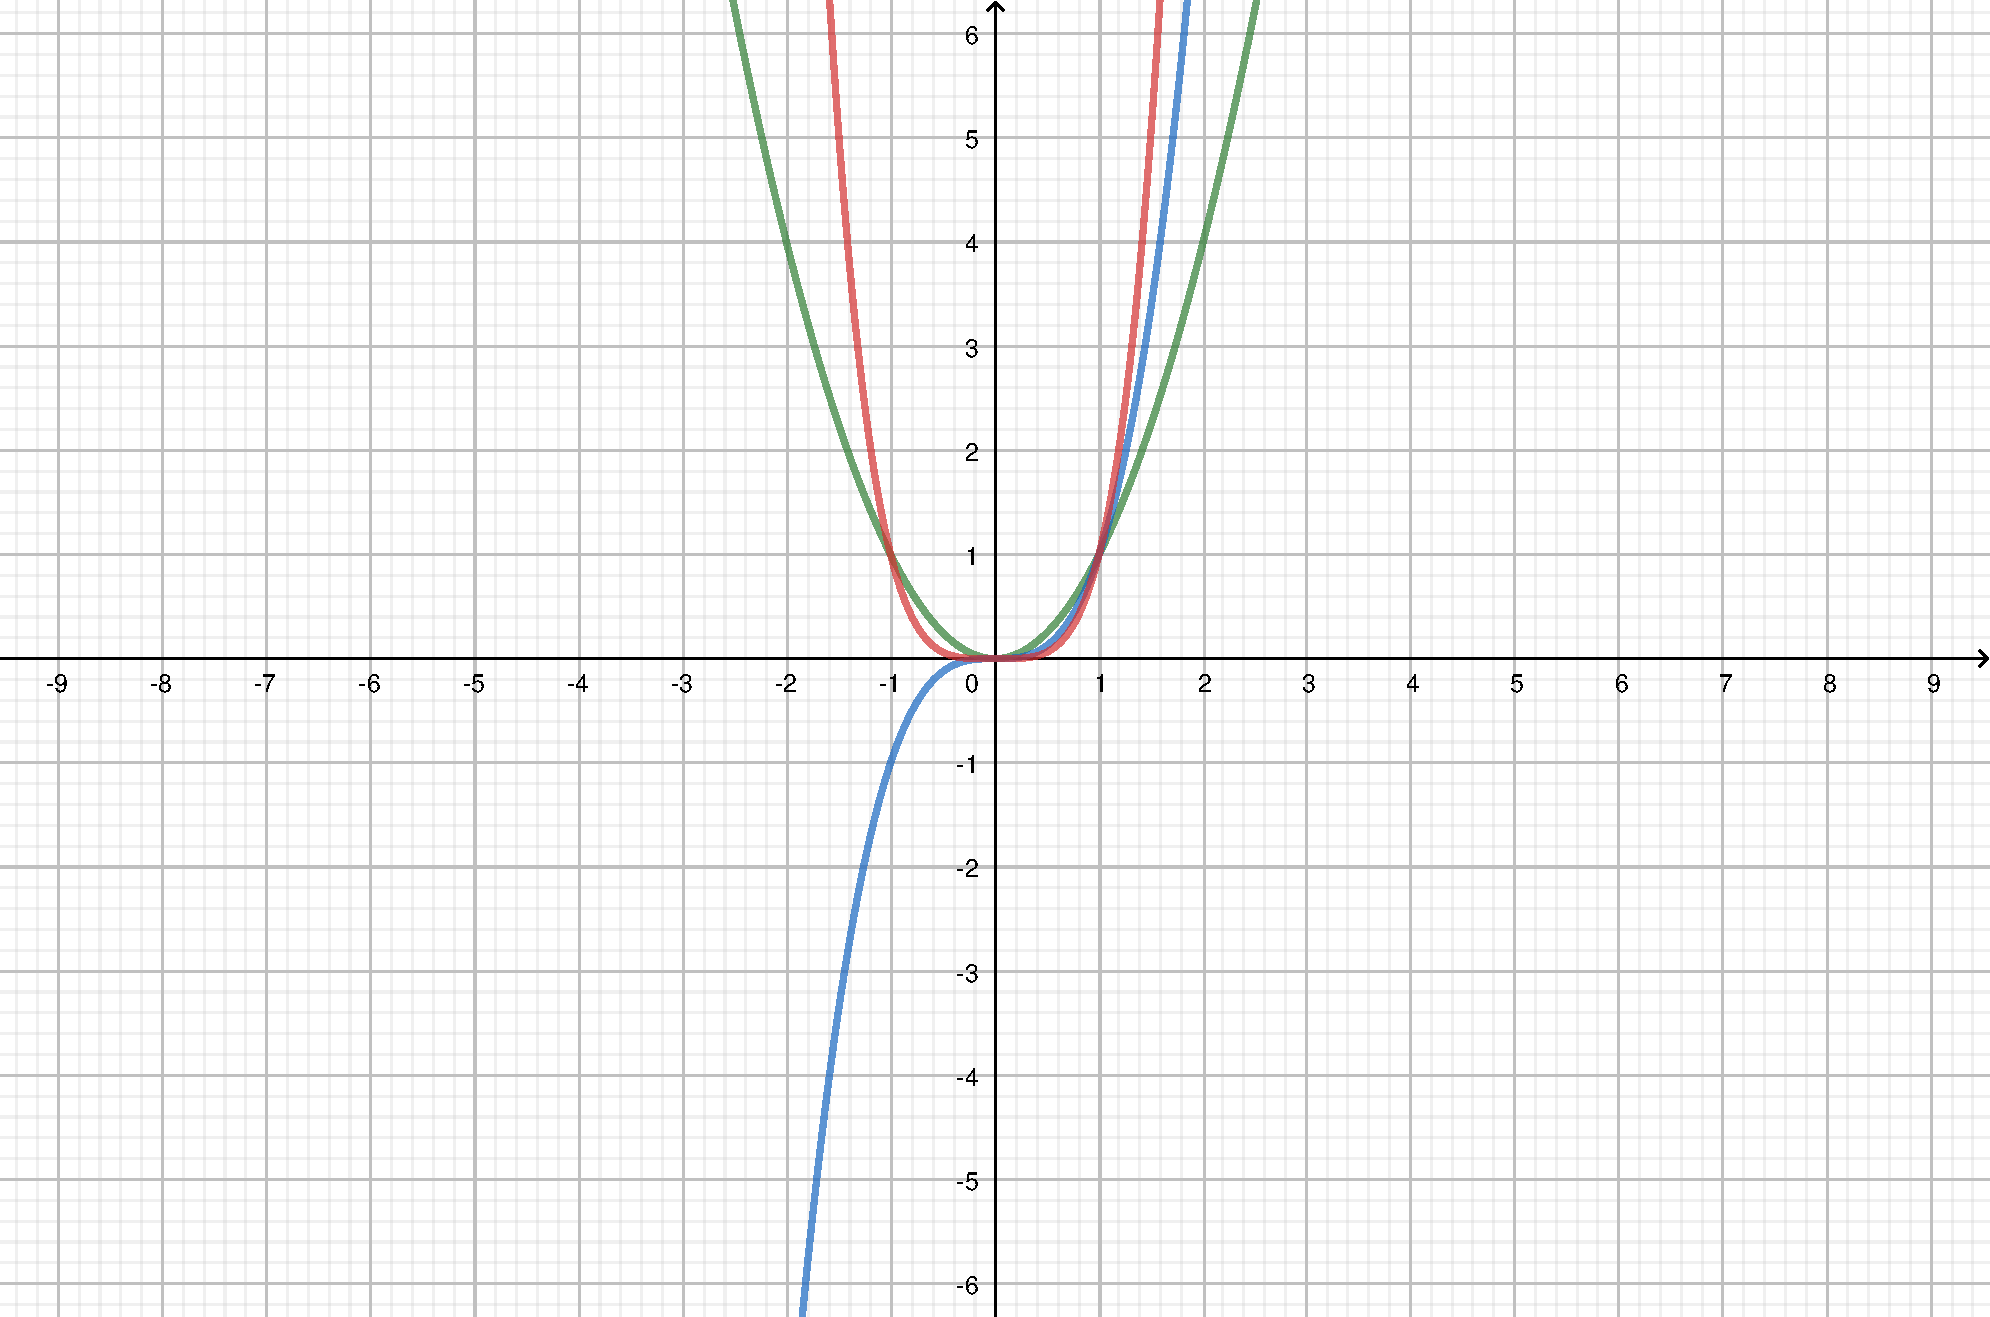
\includegraphics[width=10cm]{pdfs/gex.pdf}
  \caption{This is figure}\label{figure.x2-3-4}
\end{figure}
\end{lstlisting}

\myo
\begin{figure}[h]
  \centering
  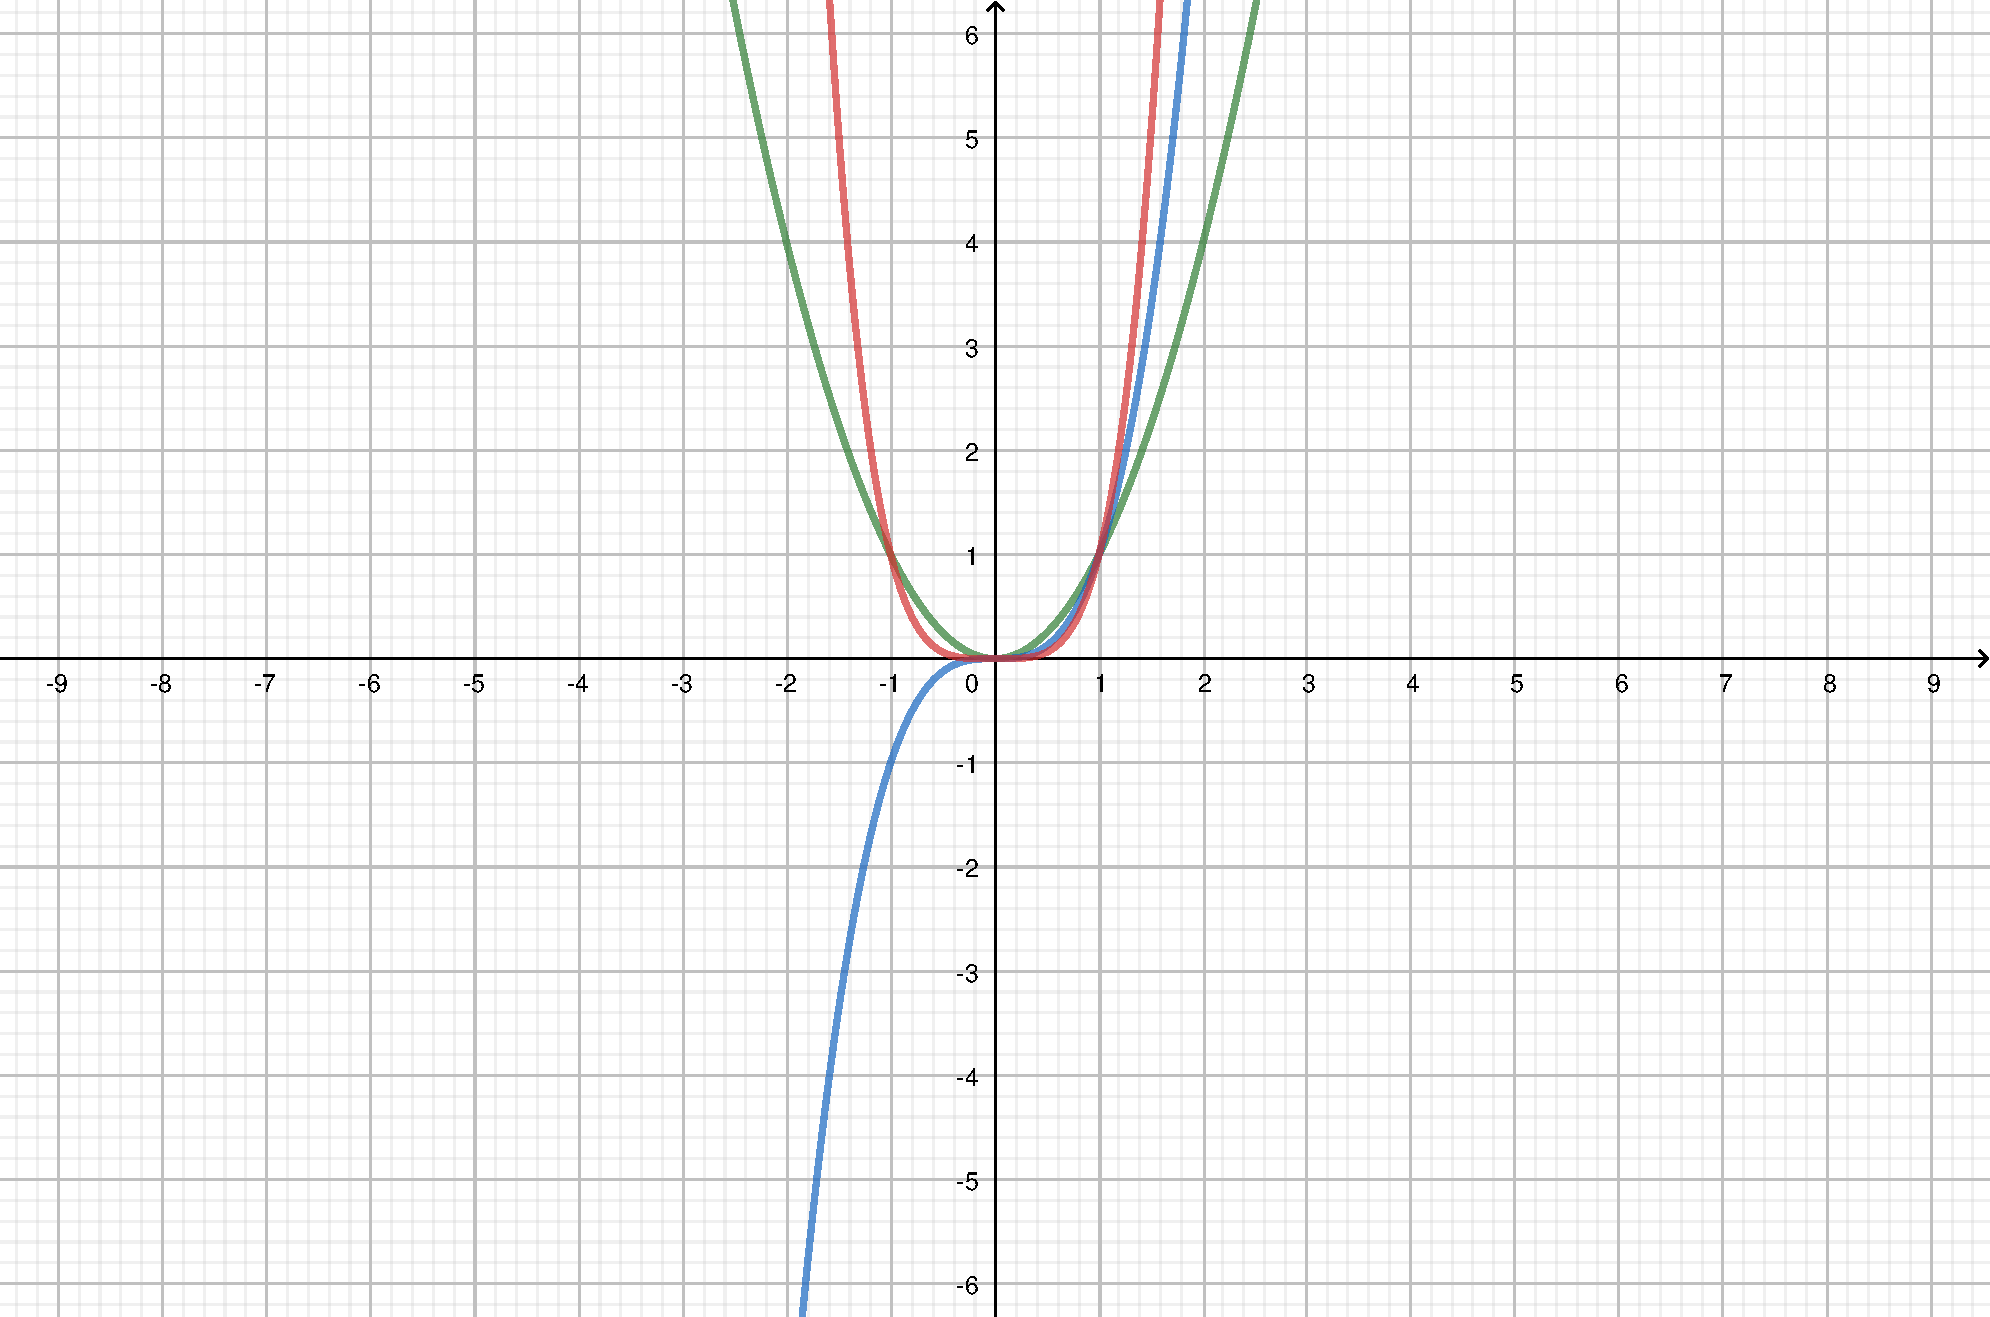
\includegraphics[width=10cm]{pdfs/gex.pdf}
  \caption{This is figure}\label{figure.x2-3-4}
\end{figure}

\myc
\begin{lstlisting}
\begin{figure}[h] % h is very important 'here'
  \centering
  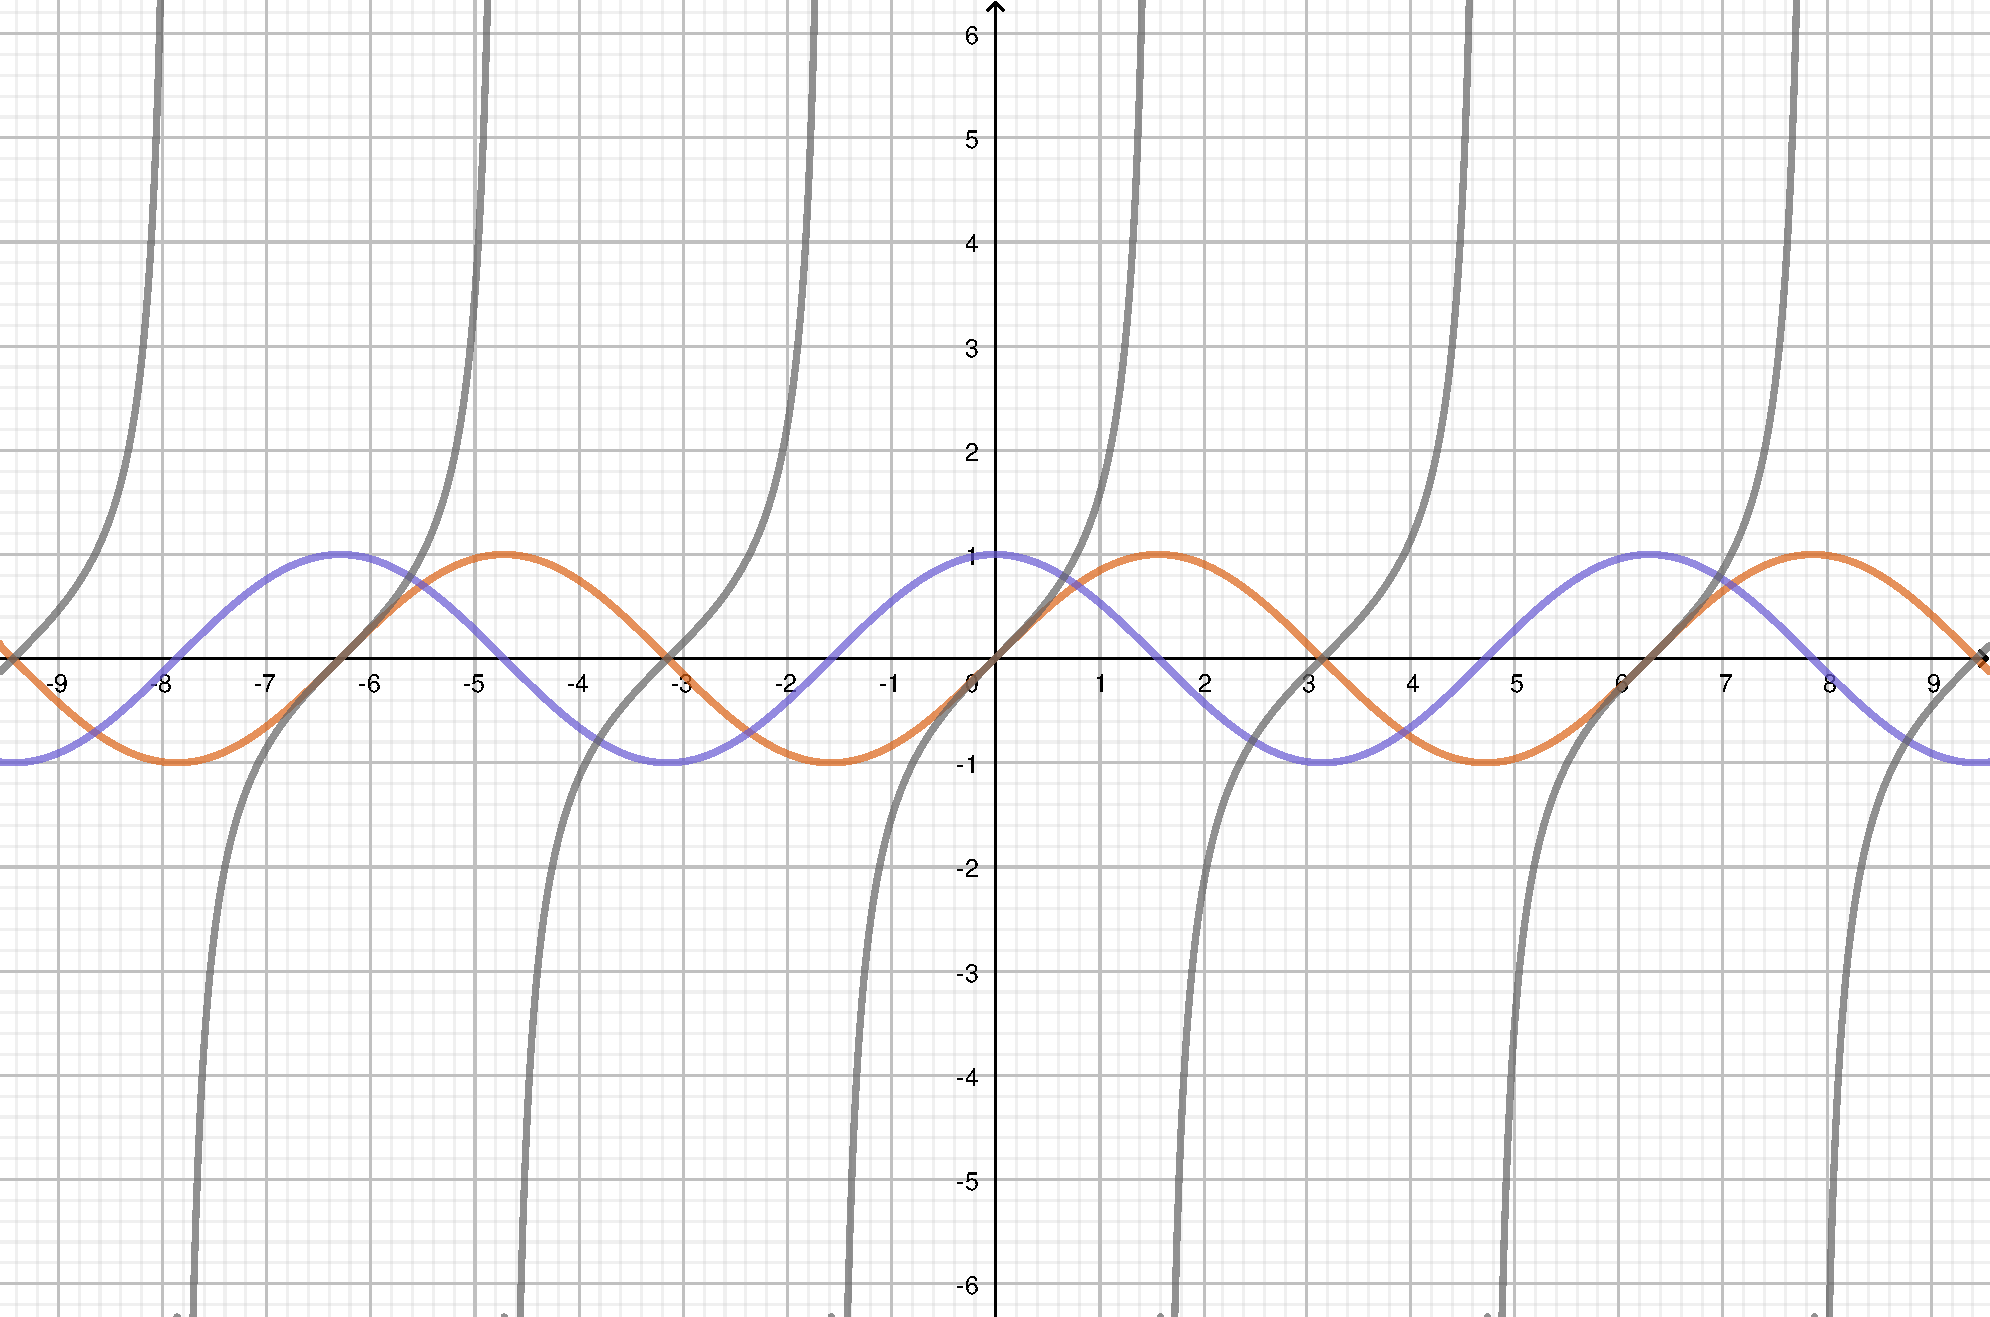
\includegraphics[scale=0.3]{pdfs/gex2.pdf}
  \caption{This is figure}\label{figure.x2-3-4}
\end{figure}
\end{lstlisting}

\myo
\begin{figure}[h]
  \centering
  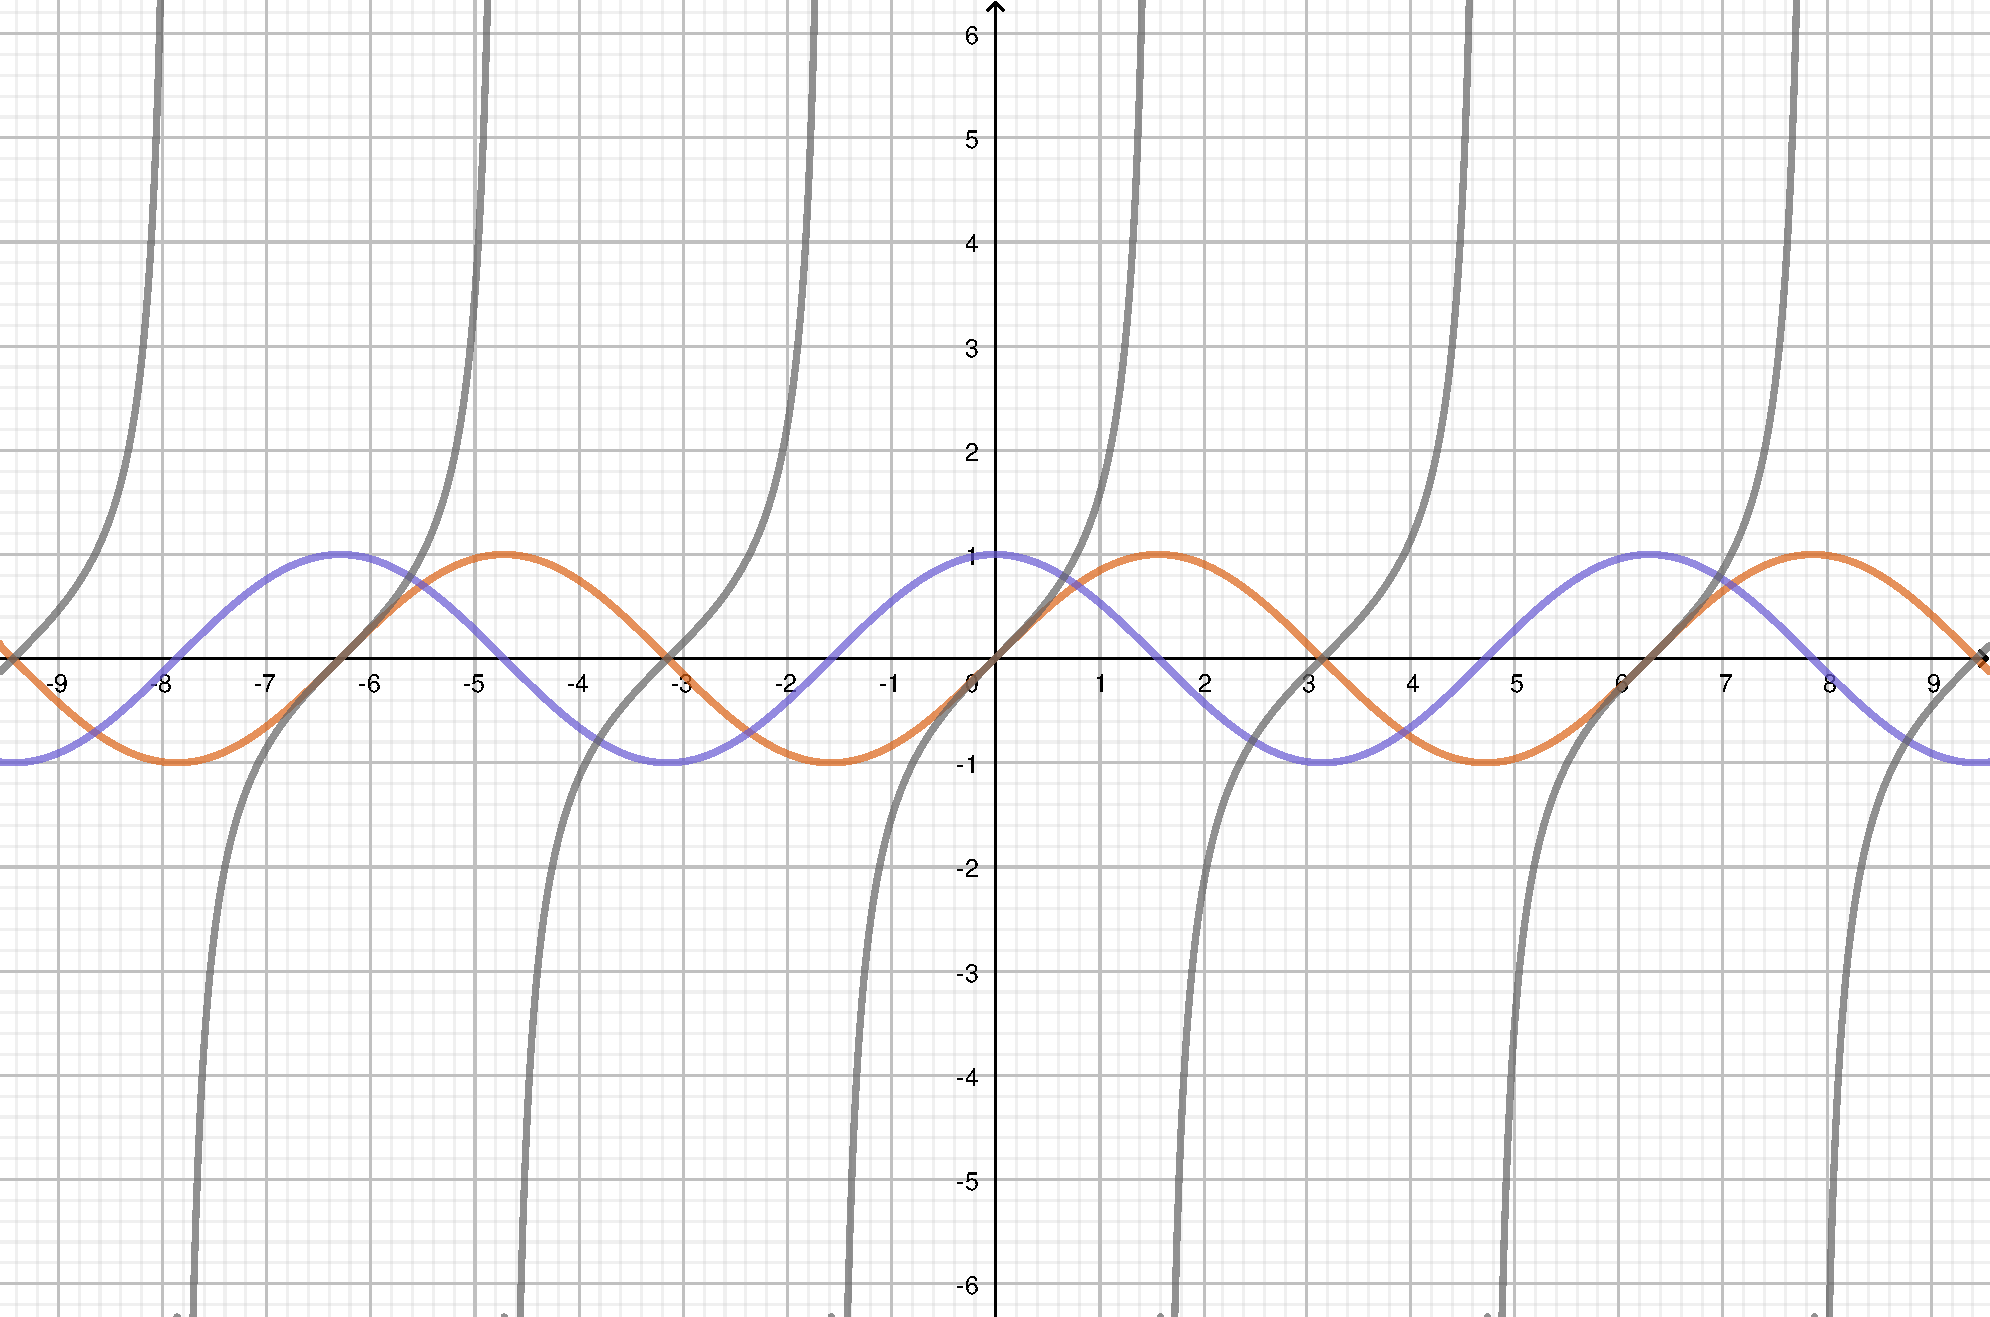
\includegraphics[scale=0.3]{pdfs/gex2.pdf}
  \caption{This is figure}\label{figure.x2-3-4}
\end{figure}

\chapter{Notes}
\section{newcommand}
\myc
\begin{lstlisting}
%%% newcommand %%%
\newcommand{\abbas}{\textcolor[rgb]{0.65,0.92,0.14}{\textbf{\emph{ABBAS}}}}
\newcommand{\myc}{\noindent\textbf{{\color{blue} Code}:}}
\newcommand{\myo}{\noindent\textbf{{\color{blue} Output}:\\}}
\newcommand{\cool}[2]{{\colorbox{black}{{\color{red} #1}, {\color{green} #2}}}}
\end{lstlisting}


\begin{lstlisting}
\abbas  is a new command! see the code! \\
\cool{ali}{abbas} is a new cool command! \\
use from it repeatedly \cool{first}{second}\\
\cool{Abbas}{Yazdanmehr}\\
\end{lstlisting}

\myo
\abbas  is a new command! see the code! \\
\cool{ali}{abbas} is a new cool command! \\
use from it repeatedly \cool{first}{second}\\
\cool{Abbas}{Yazdanmehr}\\

\section{renewcommand}
focus on the superscript\footnote{superscript}\\
renewcommand uses same syntax as newcommand.

\end{document} 